\documentclass[sigconf]{acmart}
 
\settopmatter{printacmref=false} % Removes citation information below abstract
\renewcommand\footnotetextcopyrightpermission[1]{} % removes footnote with conference information in first column
\pagenumbering{arabic}
%\pagestyle{empty}

 
\usepackage{times}
\usepackage{fancyhdr,graphicx,amsmath,amssymb}
\usepackage[ruled,vlined]{algorithm2e}
\usepackage[toc,page]{appendix}

\newtheorem{definition}{Definition}
\newcommand{\eat}[1]{}


%% end of the preamble, start of the body of the document source.
\begin{document}

%%
%% The "title" command has an optional parameter,
%% allowing the author to define a "short title" to be used in page headers.
\title{On recognizing uniform areas in a heterogeneous dataset}

%%
%% The "author" command and its associated commands are used to define
%% the authors and their affiliations.
%% Of note is the shared affiliation of the first two authors, and the
%% "authornote" and "authornotemark" commands
%% used to denote shared contribution to the research.
\author{Odysseas Papakyriakou}
\affiliation{%
  \institution{Utrecht University}
  \streetaddress{1 Th{\o}rv{\"a}ld Circle}
  \city{Utrecht}
  \country{The Netherlands}}
\email{o.papakyriakou@students.uu.nl}

\author{Thanos Tsiamis}
\affiliation{%
  \institution{Utrecht University}
  \streetaddress{1 Th{\o}rv{\"a}ld Circle}
  \city{Utrecht}
  \country{The Netherlands}}
\email{a.tsiamis@students.uu.nl}

%%
%% By default, the full list of authors will be used in the page
%% headers. Often, this list is too long, and will overlap
%% other information printed in the page headers. This command allows
%% the author to define a more concise list
%% of authors' names for this purpose.
\renewcommand{\shortauthors}{Papakyriakou and Tsiamis}
\keywords{datasets, data intensive systems, clustering}

%%
%% This command processes the author and affiliation and title
%% information and builds the first part of the formatted document.
\maketitle
\pagestyle{plain}
\pagenumbering{arabic}

\section{Introduction}
In the digital era we are living in, the amount of data people are using is increasing exponentially. According to the Statista Research Department \cite{StatistaAmountofData}, the total amount of data created and replicated in 2020 reached a new high of just over 64 zettabytes. To put this into perspective, from the beginning of the human race to the year 2003, it is estimated that 5 exabytes of data are created \cite{humanRaceDataAmount} which is only 0.5\% of a zettabyte! Data varies not only in size but also in forms and speed. These forms may include various means such as photos, videos or even random pieces of byte strings.

Meanwhile, as the Internet of Things (IoT) is gaining a lot more traction, more and more objects and devices are connected to the internet, gathering data on customer usage patterns and product performance. This rapid increase in data production has led to the use of the term "big data" \cite{5V's} to describe this new era of massive data. Although there is no clear definition of what constitutes big data, they are typically characterized by what is called the five V's: \textit{Volume}, \textit{Veracity}, \textit{Value}, \textit{Variety}, and \textit{Velocity} \cite{5V's}.

Data cannot be thought as a standalone entity. They are tightly coupled with the notion of a database, an organised collection of data, typically controlled by a Database Management System (DBMS). Specialised systems and frameworks have to be implemented to facilitate all these enormous amounts of data. Such systems, the so called data intensive systems, use state-of-the-art technologies to interact with big data in sizes that would otherwise seem prohibitive.

However, designing solutions for data intensive systems has its challenges. Decomposing a dataset into partitions such that each decomposition is highly homogeneous is one of them. Specifically, we are interested in a decomposition of a dataset $D$ to a set of datasets $D_i$, 1$\leq i \leq k$ such that the average of the homogeneities of these	sub-datasets is maximized. Homogeneity is quantified by a function described in section \ref{Solution}. An important feature of decomposing a dataset into smaller and more similar ones is the ability to identify what these smaller datasets have in common. Therefore, being able to query all elements of the same subset is of uttermost importance for the purpose of this paper.

This is a challenging task for several reasons. Firstly, the proposed solution should be dataset agnostic, meaning that it should work for any relational table, so its performance should not be dependent on the specifics of any particular dataset. Moreover, maintaining scalability while preserving performance is another important issue, since the goal is for the solution to work on very large tables.


At a first glance, one might argue that this problem is highly pointless. A database is nothing more than a collection of data; a data analyst may as well take a look into the dataset and partition it appropriately based on their background knowledge.

While the validity of this manual method has its benefits, the goal of this paper is to tackle this problem from a systems software perspective. Designing and developing a system that can split the dataset into similar subsets can have multiple benefits. By using this framework first, data scientists and experts on the field can filter the data on some initial assumptions, that of the similarity of specific attributes. Then, each split can be analysed more in depth; for example, by business analysts.

The solution followed here, is a search tree approach that is somewhat similar to that of a decision tree. In short, the database is split every time into two sub-databases where each child can be queried based on some attribute. Thus, by definition, it has always at least one attribute which is \textit{pure} (i.e. all elements in that attribute are the same). Results of these method are promising as they shows that the solution maintains speed without compromising much on the performance.

\section{Related work}
Schkolnick \cite{hsiao1977clustering} introduced a Clustering Algorithm for Hierarchical Structures which addressed how to store a hierarchic structure in order to minimize the expected access time to it. Chang and Cheng \cite{ChangCheng} presented a model for structured database decomposition based on the relational database model. In their paper, they investigated the decomposition of a database based on the \textit{decomposition tree}, a structure with nodes and edges where relations on the edges denote the steps to decompose the database. The solution proposed in this paper was heavily inspired by the algorithm in the paper by Chang and Cheng \cite{ChangCheng}.

To evaluate our proposed solution, two things are necessary: a baseline solution for comparison, and a homogeneity function that estimates how homogeneous each decomposition is. The baseline solution makes use of the K-Means algorithm \cite{lloyd1982least}. The homogeneity function is heavily inspired by the Gini impurity measure \cite{Grabmeier-2007}. The algorithm is deeply dependent on Spark \cite{spark2018apache} which is a multi-language engine for executing data engineering, data science, and machine learning on single-node machines or clusters. To increase speed and performance, Spark's dataframes were used \cite{armbrust2015spark}, a concept which evolves the notion of Spark's RDD \cite{zaharia2012resilient}, thus allowing the algorithm to run in parallel, across several nodes.

\section{Solution}\label{Solution}
As hinted before, the main algorithm constitutes of a search tree implemented in Apache Spark. However, blindly designing an algorithm without comparing it to some other well known algorithm would serve no purpose; single results would have to be displayed which wouldn't show any significance by themselves. Thus, a baseline solution to the problem is developed as well.

K-means clustering was used as a baseline solution, which is also implemented in the Spark framework and is extensively used for grouping elements in a database.

\subsection{Infrastructure}
The Spark framework was run in a Google Colab environment, which easily allows distributed computing on Google's servers. Minimal modifications to the Spark Context were done due to limitations from Google's free version. Nevertheless, the maximum amount of workers was used with the \textit{local[*]} command. Other than that, the necessary dependencies required for spark to run were set, such as setting the right HOME variable for spark and importing the correct packages.


\subsection{Transforming the database}\label{TransformingDatabase}
The database, whatever its contents might be, is not necessarily in the right format to run K-Means or our algorithm on it. Namely, the attribute values might not be all numerical. Therefore, the data were transformed with \textit{StringIndexer}, a package by Spark, which gives an increasing number for each distinct class in each attribute in the dataset. It was also assumed that the input database contains a header, or labeled column names.

For example, consider the following toy dataset: 
\begin{center}
\begin{tabular}{||c c c||} 
 \hline
 Id & Color & Shape \\ [0.5ex] 
 \hline\hline
 1 & Red& Triangle\\ 
 \hline
 2 & Red & Square\\
 \hline
 3 & Green & Circle\\
 \hline
 4 & Red & Square\\
 \hline
 5 & null & Triangle\\ [1ex] 
 \hline
\end{tabular}
\end{center}
StringIndexer then encodes the element which would transform the database into:
\begin{center}
\begin{tabular}{||c c c||} 
 \hline
 IdIndexed & ColorIndexed & ShapeIndexed \\ [0.5ex] 
 \hline\hline
 0 & 0 & 0\\ 
 \hline
 1 & 0 & 1\\
 \hline
 2 & 1 & 2\\
 \hline
 3 & 0 & 1\\
 \hline
 4 & 2 & 0\\ [1ex] 
 \hline
\end{tabular}
\end{center}

Notice that the column names are changed as well where the suffix "Indexed" exists at the end of each word. This shouldn't be of much concern and is for cleaner code practices.

Addressing the null values is the first obstacle in preprocessing the data. It was decided to treat null values as their own category and give them a special value of -999999 before encoding them with StringIndexer. This value, according to Benford's law \cite{miller2015benford}, should have the least impact.

String Indexer gives a unique value for each class in an attribute based on the frequency of the words. In the example above, "Red" gets the value 0 as it is the most common, while "id":1 gets the value 0 as it is the first one among all the id values and all id values are unique.
This method, can now encode arbitrary strings into the metric space. However, due to the fact that in each new string the StringIndexer has to check every other string to verify whether it is a new entry or not, there were some issues regarding heap space. 

\subsection{Homogeneity function}\label{HomFunction}
To measure the similarity of the items in a database a custom homogeneity function was used. 

The hom function (\textit{"hom"}) can be defined as the average $(hom\_attribute(attr))$ where $hom\_attribute$ is defined as:\begin{equation}
    hom\_attribute(attr) = \begin{cases} 0 \text{, if frequency of all elements is 1} \\ \frac{max(\text{category\_frequency})}{length(attribute)} \text{, otherwise}\end{cases} 
\end{equation}

Informally speaking, the homogeneity of a single attribute is the relative frequency of the most prevalent value. In the case where an attribute contains only unique values (e.g. UUIDs), then the homogeneity of that attribute is by definition zero. On the other hand, if all values were of a single class (e.g. Color "Red"), then the homogeneity would be 1. Therefore, the range for the homogeneity function is [0, 1]. For example, the homogeneity of Figure \ref{fig:DatasetSnippet} in the following pages, is $0.375=\frac{0+1+0+0+1+0.25}{6}$ where each number in the nominator is the homogeneity of the attribute (starting from left to right).

Regarding the actual implementation, the hom\_attribute function takes as an input a dataframe (i.e. dataset) and returns as an output the homogeneity value of that dataset alongside a dictionary of the homogeneities of each individual attribute. The reason the algorithm returns a dictionary will be explained in section \ref{OurAlgorithm}.





\subsection{Baseline solution}\label{BaselineSolution}
The most obvious solution, if someone would solve the problem of clustering, would be to use K-means clustering. K-means would cluster the data into $k$ separate fields and we would have to just compute the homogeneity of those fields based on the $k$ labels it produced. The only way to query the k clusters would be on the label alone (e.g. the points belonging to the third cluster). In short, the algorithm uses the squared euclidean distance as a distance measure and silhouette score as a metric name to produce the clusters.

Delving into specific details, implementing K-means on Spark is fairly easy. However, the transformed database described in section \ref{TransformingDatabase} is not yet in the right state.

Specifically, the data need to be further transformed into vectors in the $\mathbb{R}^d$ space where $d$ denotes the number of columns. This process is quite straightforward with the \textit{VectorAssembler} package included in Spark. A nice property of \textit{VectorAssembler} is that in case a vector contains a high percentage of zeroes, then it is transformed into a Sparse Vector, thus saving space and increasing performance.

Afterwards, $k$-clusters were computed, where $k$ ranges from 2 to 14, and their silhouette score was found. There is no straightforward way to pick the right amount of clusters and various arguments can be made for every choice. Figure \ref{fig:SilhScore} provides an example of a silhouette score plot, which often helps guide the selection of $k$. 
\begin{figure}[h!]
    \centering
    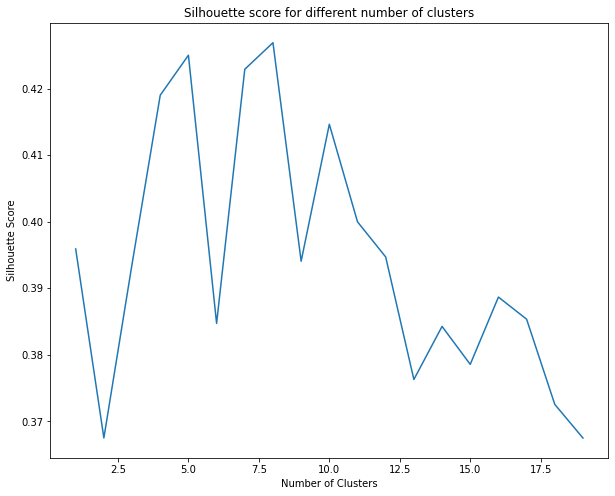
\includegraphics[scale=0.35]{images/SilhouetteScore.png}
    \caption{Silhouette Score}
    \label{fig:SilhScore}
\end{figure}

After K-means clusters the data into $k$ clusters we compute the homogeneity of each cluster with the average$(hom\_attribute(attr))$ described in section \ref{HomFunction}. Then the general homogeneity is computed as the average of those clusters. The complete code can be found in Appendix (Figure \ref{fig:HomKMeans}).

Results of the K-Means are presented in section \ref{Results}.




\subsection{Algorithm}\label{OurAlgorithm}
\subsubsection{High Level Overview:}
As explained before, the main idea of the treeGrow algorithm is that of a search tree that in each step splits the database into two sub databases and computes their homogeneity. The split is done based on a feature which has the maximum permitted homogeneity. The word \textit{permitted} is deliberately placed here as it made sense not to split the database into very small databases. After all, 1 tuple databases could be queried perfectly and would have homogeneity of 1 but it wouldn't make any sense to be a distinct decomposition. Thus, users of the program can set their own hard limit (called \textit{HARD\_LIMIT}),  a number which the algorithm would stop if found itself with less than those rows.

Figure \ref{fig:ourAlgoExample} contains a visual example of this novel algorithm. In that example, the original database is split into two parts based on the max frequency value of the third column and then (for the left child) on the max frequency value of the first column. Rectangles denote the leaves of the tree. The prohibition sign indicates that hard limit forbids the database to split into sub-databases as they would create children with less than HARD LIMIT rows. To get the SQL-queries of the leaves we have to traverse the tree from the root to the leaves. The leaves are tagged with a specific boolean value to distinct them from the other nodes in the output. We omit the tree traversal algorithm from the main implementation as we believe it is out of the scope of this paper. 


\begin{figure}[h!]
    \centering
    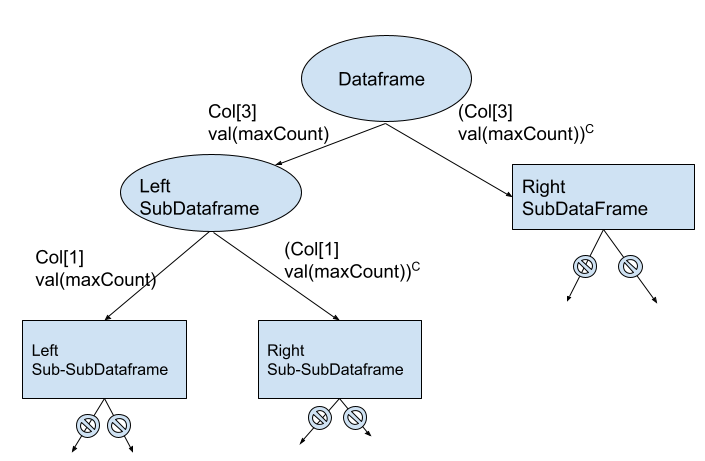
\includegraphics[scale=0.36]{images/TreeFigure.png}
    \caption{Example of the splitTree algorithm}
    \label{fig:ourAlgoExample}
\end{figure}

Algorithm \ref{treeGrow} provides some pseudocode for what the algorithm is doing. The key point of the algorithm is the working\_list which is nothing more than a queue keeping track of the elements added. When the queue is empty, it means that no more elements (i.e. sub-dataframes) are to be processed, so the tree process is complete. In a random step $k_r$ of the algorithm, for the head of the queue, it computes the homogeneity of each attribute of the dataframe and it passes this result to a list which is reordered in a descending fashion.

Given the (ordered) list returned by the hom function, the algorithm searches to see if there is a split which, when done, does not violate the hard limit constraint. If there is no such constraint, then this means that the dataframe has no other choice than to be a leaf. If there is, then it searches for the most frequent value and splits based on that. By construction, the left child will always have the equality of that value, while the right the inequality.



\begin{algorithm}[h!]
\SetAlgoLined
\KwResult{A list containing the nodes of the tree}
 working\_list=[root\_node]\;
 tree=[]\;
 HARD\_LIMIT=compute\_hard\_limit()\;
 \While{working\_list is not empty}{
  current\_node = first element in the working\_list\;
  remove first element in the working\_list\;
  (hom\_val,hom\_atr\_list) = compute hom of the dataframe\;
  ordered\_hom\_atr = order hom\_atr\_list map in desc homogeneity\;
  isLeaf = True \;
  
  \For{each attribute in ordered\_hom\_atr}{
  \If{it can pass the HARD LIMIT constraint}{
   value = groupBy this attribute for the most frequent value\;
   left\_child = dataframe filtered where attr == value\;
   right\_child = dataframe filtered where attr != value\;
   working\_list.append(left\_child)\;
   working\_list.append(right\_child)\;
   tree.append(current\_node)\;
   isLeaf = False\;
   break from the for Loop\;
   }
   \If{isLeaf is True}{
   tree.append(current\_node)\;}
   }
 }
 return tree\;
 \caption{TreeGrow Algorithm}\label{treeGrow}
\end{algorithm}







\subsubsection{Implementation details}

The following section describes the implementation details of the aforementioned algorithm in depth. It is implemented mainly in \textit{Python} with \textit{PySpark}.
Since the main concern is dealing with big data, the data structures used are mostly either PySpark DataFrames or in some fewer cases PySpark RDD's. For cleaner code practises, most of the functions related to the treeGrow algorithm are wrapped up inside a class.

Arguably, the hom\_atr\_list is one of the costliest operations in the whole program. It uses map reduce technologies to count the most frequent value in each attribute and then expresses it as a percentage relative to the other values. Algorithm \ref{HomSample} gives a small sample of the hom process. While its syntax may be complex, its difference in performance in comparison to pure Python is immense. The hom function returns a tuple with two things. The first is the hom value of the dataframe (e.g. 0.65), while the second argument returns a map which contains the homogeneity of each attribute. The reason for the second return is purely for convenience and performance. The whole function can be found in Appendix \ref{HomFunctionAppendix} (Figure \ref{fig:FullHomRdd}).


To easily keep track of the relations between the parent and the children each node is a class named Node which contains the following instance variables:  \textit{df}, \textit{feature}, \textit{left\_child}, \textit{right\_child}, \textit{hom\_measure} and \textit{leaf}. Variable df is the dataframe which this specific node pertains to. Variable feature is the attribute the two children were split on. In the case of leaves, the variable is empty. The variables left\_child and right\_child keep track of the relationships between the parent and the children. In that way, the user can traverse the tree easily to find the SQL command for a desired leaf. The hom\_measure keeps track of the dataframe's homogeneity score while the leaf variable is a boolean structure which verifies whether this particular node is a leaf or not.


\begin{algorithm}[h!]

 x = df\_new.rdd.groupByKey() \textbackslash\\
                            .mapValues(list) \textbackslash\\
                            .map(lambda x: (x[0], Counter(x[1]).most\_common(1)))\textbackslash\\
                            .map(lambda x: (x[0], x[1][0][1])) \textbackslash\\
                            .map(lambda x: (x[0], x[1] if x[1] > 1 else 0))\textbackslash\\
                            .map(lambda x: (x[0], x[1]/nrows))\;
 \caption{Homogeneity Sample}\label{HomSample}
\end{algorithm}

\section{Experimental evaluation}

\subsection{Datasets}
Three kinds of datasets were considered for the experiments: \textit{Small}, \textit{Medium} and \textit{Large}. Small is the well known titanic dataset which describes the survival status of individual passengers
on the Titanic. Titanic dataset contains 891 entries.

Medium and Large are samples from title.basics.tsv.gz IMDB database which contains over 9 millions entries related to the movie industry\footnote{The database can be found at \href{https://www.imdb.com/interfaces/}{https://www.imdb.com/interfaces/}}. When sampling the full dataset to create the smaller datasets, a seed was set to the value of 111 to ensure repeatability of the results.

Medium database contained 0.001 of the original database (8,978 entries) while Large contained 0.01 of the original database (90,141 entries).

A snippet of the medium dataset can be seen in Figure \ref{fig:DatasetSnippet}.
\begin{figure}[h!]
    \centering
    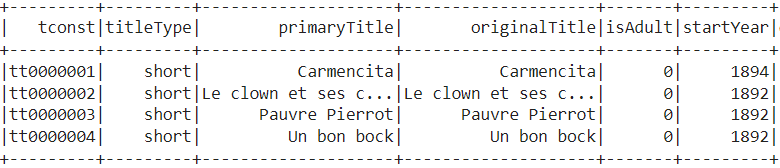
\includegraphics[scale=0.4]{images/DatabaseSnippet.png}
    \caption{Dataset Snippet}
    \label{fig:DatasetSnippet}
\end{figure}
The dataset contains other attributes as well, which due to space constraints are not included in the figure. A snippet of the small dataset can be found in Appendix (Figure \ref{fig:SmallDatabaseSnippet}).


\subsection{Results}\label{Results}
All experiments shown in the main paper have been conducted on the medium dataset. Other experiments can be found in the Appendix section.

Figure \ref{fig:SilhScore} presented above, shows the silhouette score for various $k$ values. 

In treeGrow we have no direct control of the amount of sub-datasets (i.e.leaves) the algorithm will create. Adjusting the hard limit to higher values will obviously create at most as many as the previous lower value but there are no guarantees for the specific amount. The only direct comparison between the K-means and the treeGrow algorithm would be about how the homogeneity fluctuates based on the hyperparameters of the problem. In the case of treeGrow, the hyperparameter would be the hard limit while in $k$-Means the number of clusters. 
Figure \ref{fig:medium_data} shows exactly that.
\begin{figure}
    \centering
    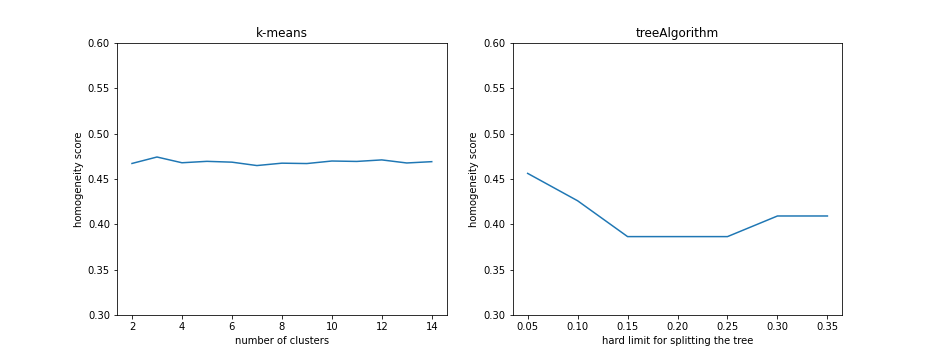
\includegraphics[scale=0.28]{images/medium_dataset.png}
    \caption{Comparing KMeans with treeGrow}
    \label{fig:medium_data}
\end{figure}

Figure \ref{fig:HomAmountOfLeaves} shows the homogeneity score relative to the hard limit with the number of leaves appended to each point in the graph. Notice how a strict hard limit (in this case 0.05) improves the homogeneity score while a more lenient one (e.g. 0.25) decreases it. There is no strictly defined rule on finding the best hard limit on a dataset. We leave it to the kind discretion of the user to choose their desired threshold. As a rule of thumb, we believe that values around 12\% maintain a moderate amount of leaves while keeping the homogeneity score relatively high.
\begin{figure}
    \centering
    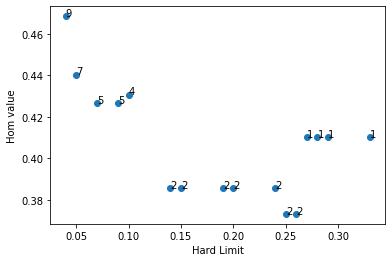
\includegraphics[scale=0.55]{images/HomVsAmountOfLeavesForMedium.png}
    \caption{Homogeneity score for treeGrow algorithm}
    \label{fig:HomAmountOfLeaves}
\end{figure}

In order to measure how long each command took, we used the $\%\%timeit$ command which measures how long each cell in the notebook takes to run by reiterating it 5 times and taking the average. Commands pertaining to the same functionality were grouped together in the same cell. Naturally, this system isn't impervious to objections but it shows a general approximation of the time it took.

Figure \ref{fig:TimeComp} shows the running time in seconds. This graph by no means acts a way to compare the algorithms timewise. That would be pointless, since a range of few strict hard limits cannot be compared to a range of some $k$ for K-Means. Our purpose is to show, in general, the running times which should act as a guideline to the problem's general time complexity. 
\begin{figure}[h!]
    \centering
    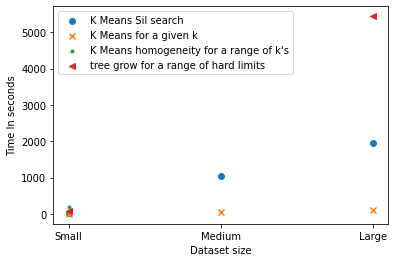
\includegraphics[scale=0.4]{images/TimesComparisons.png}
    \caption{Time it took to run various algorithms}
    \label{fig:TimeComp}
\end{figure}

\section{Discussion}
A few points are noteworthy when looking at the results. Figure \ref{fig:medium_data} shows approximately a 10\% reduction in the homogeneity value for the same amount of decompositions between kMeans and treeGrow. However, we argue that this is not the whole picture. 

In the worst case, the algorithm will create half of the nodes (right children) in which their homogeneity may be as low as possible. These children, even though they lack one common value for a give feature,  they are similar in another sense; their values for the attribute based on which the split was made are all different from the value of the most common feature. Hence, everything can be queried not based on the label of the cluster they are in, but by something more powerful, that of the belongingness (or not) in an attribute.

On the other hand, K-means, albeit its higher hom values, it provides nothing more than a label for each of the entries. As a result, the clusters have to be processed again to examine their common point (if one exists at all).

To make this notion more concrete, consider the following example. A movie streaming platform offers 4 kinds of subscriptions for its customers: basic, premium, gold and diamond. Assume in its most simple form that the algorithm splits the database in two cases. That of those that have purchased the basic subscription and those who haven't. The hom function of this split in the worst case would be $\frac{1+0}{2} = 0.5$. The right child, albeit its homogeneity score of 0, can still be considered in a way fully homogeneic as those elements can be queried where subscription is not basic. As a result, the Data analytics team can take full advantage of this split and run an ad campaign on the relevant clientele.




As a future work, we would like to make use of Spark's internal packages, namely decision trees which are optimised as best as possible. In addition to that, we would like to explore other options as a hom\_attr function. Finally, regarding the StringIndexer, we would like to look into ways to parse the database without running out of memory when the amount of data is more than a few millions.

\section{Conclusion}
A decision-tree-like novel algorithm is presented which splits the database into $n$ parts where $n$ denotes the number of leaves. The algorithm is compared to a baseline solution (K-means) which classifies the data into $k$-clusters.

The splits of the tree are well defined in two ways: the parts are distinct; that means they don't contain overlaps (i.e. duplicate elements) and they can be queried exactly. Due to the second part, the average homogeneity of the algorithm is lower than that of $k$-means. However, we argue that this number is not the alpha and omega of the problem. Being able to query the decomposition of the dataset is very important and is not feasible when using $k$-means clustering.

%%
%% The acknowledgments section is defined using the "acks" environment
%% (and NOT an unnumbered section). This ensures the proper
%% identification of the section in the article metadata, and the
%% consistent spelling of the heading.
\begin{acks}
The second author would like to thank the first author for his amazing coding skills that really helped us in difficult times. He would also like to thank Kevin from Oh{\o}j, for his amazing coffee that kept him going during this assignment. The first author would like to thank the second author for his rigorous efforts in writing this report and for an amazing collaboration.
\end{acks}

%%
%% The next two lines define the bibliography style to be used, and
%% the bibliography file.
\bibliographystyle{ACM-Reference-Format}
\bibliography{bibliography}

%%
%% If your work has an appendix, this is the place to put it.
\appendix

\begin{appendices}


\section{Databases}
A snippet of the Titanic database (i.e. \textit{small}). The snippet is taken after processing the null values to -999999. Other attributes exist as well but due to space constraints were omitted.
\begin{figure}[h!]
    \centering
    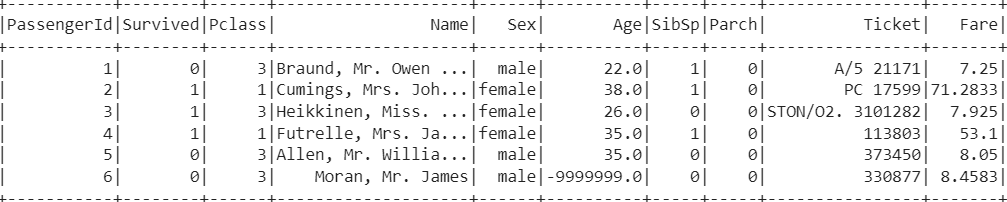
\includegraphics[scale=0.4]{images/SmallDatabaseSample.png}
    \caption{Snippet from the small Database}
    \label{fig:SmallDatabaseSnippet}
\end{figure}

\section{Experiments}
\subsection{Small Dataset}
\begin{figure}[h!]
    \centering
    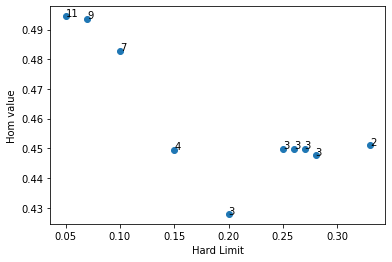
\includegraphics[scale=0.52]{images/HomVsAmountOfLeavesForSmall.png}
    \caption{Homogeneity and amount of leaves created}
    \label{fig:HomLeavesSmall}
\end{figure}

\section{Implementation Details}
\newpage
\subsection{Hom function} \label{HomFunctionAppendix}
\subsubsection{}
The homogeneity function that takes advantage of Spark's Map Reduce functions.
\begin{figure}[h!]
    \centering
    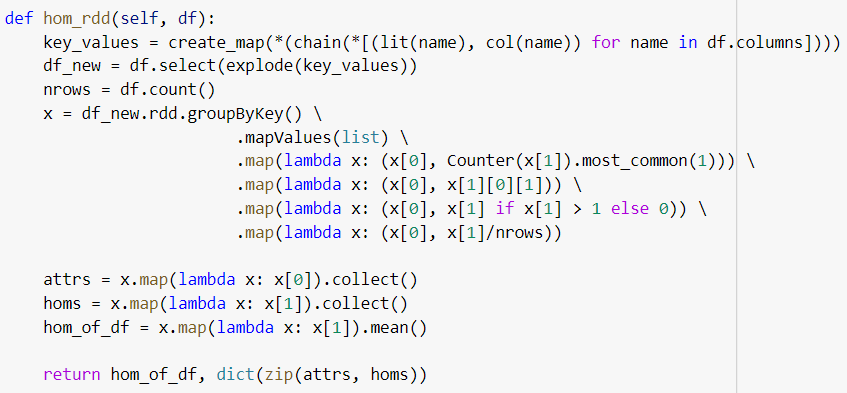
\includegraphics[scale=0.52]{images/Full_Hom_Rdd.png}
    \caption{Homogeneity function}
    \label{fig:FullHomRdd}
\end{figure}

\subsubsection{}
The homogeneity used to compute the homogeneity for k clusters from K Means
\begin{figure}[h!]
    \centering
    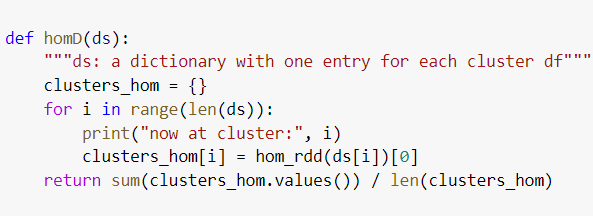
\includegraphics[scale=0.4]{images/HomKMeans.png}
    \caption{Homogeneity function for K Means}
    \label{fig:HomKMeans}
\end{figure}
\end{appendices}
\end{document}
\endinput

%%
%% End of file `sample-sigconf.tex'.
